\documentclass{article}
\usepackage[utf8]{inputenc}
\usepackage[T1]{fontenc}
\usepackage[utf8]{inputenc}
\usepackage{lmodern}
\usepackage[a4paper, margin=1in]{geometry}
\usepackage{graphicx}
\graphicspath{ {./images/} }

\usepackage{minted}
\large
\title{CSE 344 Midterm}
\begin{document}
\begin{titlepage}
	\begin{center}
    \line(1,0){300}\\
    [0.65cm]
	\huge{\bfseries CSE344 Midterm}\\
	\line(1,0){300}\\
	\textsc{\Large Processes and semaphores}\\
	\textsc{\LARGE A Producer Consumer Solution}\\
	[5.5cm]     
	\end{center}
	\begin{flushright}
		\textsc{\Large Hüsnü AKÇAK\\161044112}\\
		[0.5cm]
	
	\end{flushright}
\end{titlepage}

\section*{Program Setup}
\subsection*{Shared Memory Segment}
\begin{minted}[frame=lines, linenos, fontsize=\large]
{c}
struct ShmStatic* shmStatic; // conditional vars and unnamed semaphores
char *shmBuff;  // vaccine buffer
struct Citizen* shmCitizens; // to invite citizens to the clinic
int *shmChildPids; // to be able to send signal between any processes
\end{minted}

\subsection*{Structs}
\begin{minted}[frame=lines, linenos, fontsize=\large]
{c}
struct ShmStatic {      
    int buffSize,           // current number of vaccine                
        buffCapacity,       // vaccine buffer capacity
        totalNumOfCitizens, 
        leftCitizens,       // remaining citizen
        terminate, // a sign for others to terminate
        leftNurses,// to know which nurse prints their termination message
        vaccinationSession, // t*c
        sigIntArrived;      // to tell the other proc that SIGINT is received

    sem_t semEmpty, // initial value is buffer capacity
        semCitizenAvailable, // num of citizens waiting to be invited
        shmLock,    // lock all shared memory segment
        semVacc1,   // to notify and wait Vaccine '1'
        semVacc2,   // to notify and wait Vaccine '2'
        semVaccAvailable;  // at least a pair of '1' and '2' is available
};

struct Citizen{
    int pid;
    char gone,      // citizen leaved 
         inClinic;  // currently busy in clinic
};
\end{minted}

\subsection*{Intoduction}
    At the begining, parent process prepares shared memory segment, opens the input file, establishes signal handlers for SIGUSR1 and SIGINT. Then fork children in this order, citizens, nurses, vaccinators, pushers.
    While forking citizens, fills "shmCitizens" array as citizen pid's are going to be ascending order.  
    During the execution of the program parent process acts as "PusherV2" and at the end destroys semaphores, performs munmap and unlink for shared memory segment, wait for children then terminate.

\subsection*{File reading}
    Nurses use the same fd to read input file, it is assumed there are enough '1' and '2' pairs of shot. While reading the file irrelavent characters(other then '1' and '2') are ignored. 

\subsection*{Nurse}
    The syscronization among nurses on input file is solved with flock(), each nurse take the "LOCK EX" and when she finishes her transportation gives the lock with "LOCK UN". 
    When a nurse puts '1' into the buffer she also posts "semVacc1", if '2' is delivered "semVacc2" is posted.
    When EOF is encountered they terminated one by one, the last nurse print nurses termination message then she also gone.
    
\subsection*{Pusher V1}
    Waits for "semVacc1" in the number of expected time. When vaccine '1' is received it controls existence of vaccine '2' in the buffer if it exist post "semVaccAvailable" this means a complete shot is ready. 
    
\subsection*{Pusher V2}
    Pusher V2 follows the same steps with Pusher V1 in reverse. 

\subsection*{Vaccinator}
    Each vaccinator knows how many dose are going to be applied in total and follows the current remaining dose from shared memory segment. Until this count reaches zero they wait for vaccine '1' and vaccine '2' pairs by waiting "semVaccAvailable". When there is at least one vaccine pair the vaccinator removes them from the buffer (while having "shmLock"). Waits for "semCitizenAvailable" and invites the oldest one of them, vaccinate the citizen and post "semEmpty" for buffer two times. Then goes back start of the loop, and continues until total shots are applied.
\subsection*{ How to choose and invite the oldest citizen? }
     The array, "shmCitizens" keeps all citizens in ascending order by their process ids. Also, it is observable through this array whether the citizen leaves the clinic or is being vaccinated right now in the clinic. In the light of this this information, the oldest available citizen is invited by sending SIGUSR1 to him. 
\subsection*{SIGUSR1 setup}
    To be able to communicate with citizens through SIGUSR1 first sigprocmask is used to block the signal, after wards sigsuspend is used in citizen code to wait an invitation from a vaccinator.
\subsection*{Citizen}
    Every citizen has a while loop which is executed t times as soon as the loop starts, SIGUSR1 is being waited by sigsuspend. When the signal is arrived the citizen takes her dose, if she gets vaccinated "t" times she leaved the clinic, otherwise she post semCitizenAvailable then waits to be invited again.
    
    In general it is challenging to deal with signals, but in this scenario the signal is send by the vaccinator while he have a lock, it is guaranteed that only one signal is arriving to the same citizen at a time. 

    
\section*{Screen Shots}
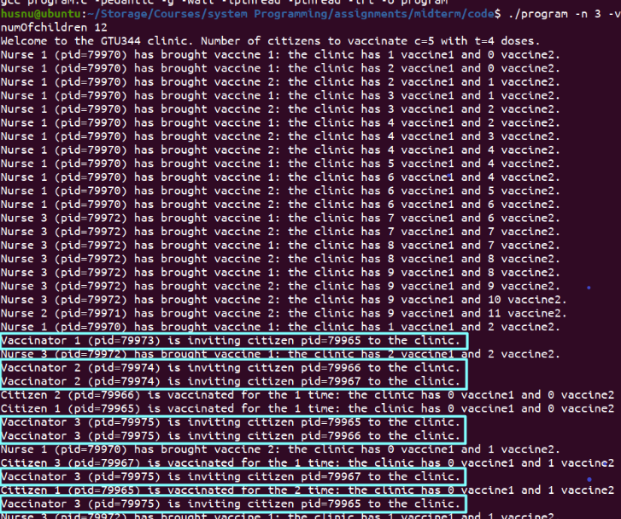
\includegraphics[]{start.png}
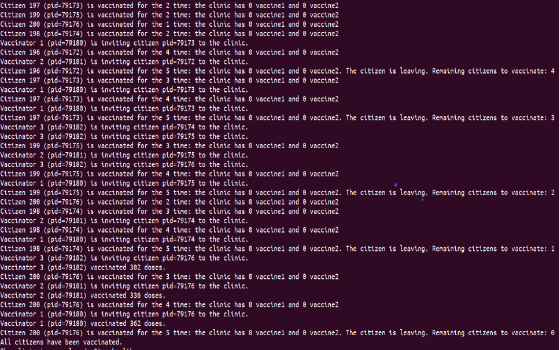
\includegraphics[]{end.png}



\end{document}











